
% v2-acmsmall-sample.tex, dated March 6 2012
% This is a sample file for ACM small trim journals
%
% Compilation using 'acmsmall.cls' - version 1.3 (March 2012), Aptara Inc.
% (c) 2010 Association for Computing Machinery (ACM)
%
% Questions/Suggestions/Feedback should be addressed to => "acmtexsupport@aptaracorp.com".
% Users can also go through the FAQs available on the journal's submission webpage.
%
% Steps to compile: latex, bibtex, latex latex
%
% For tracking purposes => this is v1.3 - March 2012
\documentclass[prodmode,acmtecs]{acmsmall} % Aptara syntax
\usepackage[spanish,polish]{babel}
\usepackage[T1]{fontenc}
\usepackage{fancyvrb}
\usepackage{graphicx,hyperref}
\newcommand\cutout[1]{}


\usepackage[table]{xcolor}
\usepackage[utf8]{inputenc}
\usepackage[parfill]{parskip}
\usepackage{tabulary}
\PassOptionsToPackage{hyphens}{url}
\usepackage{hyperref}    
\usepackage[capitalize]{cleveref}


% Metadata Information
% !!! TODO: SET THESE VALUES !!!
\acmVolume{0}
\acmNumber{0}
\acmArticle{CFP}
\acmYear{0}
\acmMonth{0}

\newcounter{colstart}
\setcounter{page}{4}

\RecustomVerbatimCommand{\VerbatimInput}{VerbatimInput}%
{
%fontsize=\footnotesize,
fontfamily=\rmdefault
}


\newcommand{\UnderscoreCommands}{%\do\verbatiminput%
\do\citeNP \do\citeA \do\citeANP \do\citeN \do\shortcite%
\do\shortciteNP \do\shortciteA \do\shortciteANP \do\shortciteN%
\do\citeyear \do\citeyearNP%
}

\usepackage[strings]{underscore}



% Document starts
\begin{document}


\setcounter{colstart}{\thepage}

\acmArticle{CFP}
\title{{\huge\sc SIGLOG Monthly 250}

 June 2024}\author{ELLI ANASTASIADI\affil{Uppsala University, SE}\vspace*{-2.6cm}\begin{flushright}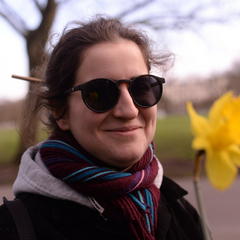
\includegraphics[width=30mm]{elli_anastasiadi.png}\end{flushright}}\begin{abstract}June 2024 edition of SIGLOG Monthly, featuring deadlines, calls and community announcements.
\end{abstract}


\maketitlee

\href{https://lics.siglog.org/newsletters/}{Past Issues}
 - 
\href{https://lics.siglog.org/newsletters/inst.html}{How to submit an announcement}
\section{Table of Contents}\begin{itemize}\item DEADLINES (\cref{deadlines}) 
 
\item CALLS 
 
\begin{itemize}\item SEFM24 (CALL FOR PAPERS) (\cref{SEFM24})
\item LPNMR 2024 (CALL FOR PAPERS) (\cref{LPNMR2024})
\item LAMAS\&SR 2024 (CALL FOR PAPERS) (\cref{LAMASSR2024})
\item FSEN 2025 (CALL FOR PAPERS) (\cref{FSEN2025})
\item FSCD 2024 (CALL FOR PARTICIPATION) (\cref{FSCD2024})
\item CAV 2024 (CALL FOR PARTICIPATION) (\cref{CAV2024})
\end{itemize} 
\end{itemize}\section{Deadlines}\label{deadlines}\rowcolors{1}{white}{gray!25}\begin{tabulary}{\linewidth}{LL}IJCAR 2024:  & Jun 04, 2024 (Early registration), Jun 24, 2024 (Late registration) \\
SEFM24:  & Jun 07, 2024 (Abstract), Jun 14, 2024 (Paper) \\
Lipari Summer School on Abstract interpretation:  & Jun 15, 2024 (Registration deadline) \\
CAV 2024:  & Jun 15, 2024 (Registration deadline) \\
LPNMR 2024:  & Jun 21, 2024 (Paper registration), Jun 28, 2024 (Submission deadline) \\
ACKERMANN AWARD 2024:  & Jul 01, 2024 (Deadline for nominations) \\
LAMAS\&SR 2024:  & Jul 17, 2024 (Paper  deadline) \\
FSEN 2025:  & Oct 07, 2024 (Abstract Submission), Oct 14, 2024 (Paper Submission) \\
\end{tabulary}
\section{SEFM24: 22nd International Conference on Software Engineering and Formal Methods}\label{SEFM24}  4-8 November 2024 University of Aveiro, Portugal\\ 
  \href{https://sefm-conference.github.io/2024/}{https://sefm-conference.github.io/2024/}\\ 
CALL FOR PAPERS 

\begin{itemize}\item  OVERVIEW  
 
  The conference aims to bring together researchers and practitioners from academia, industry and government, to advance the state of the art in formal methods, to facilitate their uptake in the software industry, and to encourage their integration within practical software engineering methods and tools. The 21st edition of the International Conference on Software Engineering and Formal Methods will be held between 6 and 8 November 2024, with workshops taking place on 4 and 5 November 2024. 
 
\item  TOPICS OF INTEREST 
 
  For a full list of the relevant topics visit the SEFM24 website.  
 
\item  IMPORTANT DATES 
 
\rowcolors{1}{white}{gray!25}\begin{tabulary}{\linewidth}{LL}Abstract submission:  & 7 June 2024 (AoE) \\
Paper submission:  & 14 June 2024 (AoE) \\
Author notification:  & Aug 15, 2024 \\
Workshops:  & Nov 4-5 2024 \\
Conference:  & Nov 6-8 2024 \\
\end{tabulary}
 
\item  INVITED SPEAKERS  
 
\begin{itemize}\item  Luís S. Barbosa, University of Minho, PT
\item  Paula Herber, Universitat Munster, DE
\item  Aleks Kissinger, University of Oxford, UK
\end{itemize} 
\item  SUBMISSION INFORMATION 
 
  We solicit two categories of papers: 
 
\begin{itemize}\item  Regular papers - describing original research results, case studies, or surveys, should not exceed 16 pages (excluding bibliography of at most two pages).
\item  Tool papers - that describe an operational tool and its contributions should not exceed 8 pages.
\end{itemize} 
  Papers must be formatted according to the guidelines for Springer LNCS papers. All submissions must be original, unpublished, and not submitted concurrently for publication elsewhere. Papers can be submitted through Easychair: \href{https://easychair.org/conferences/?conf=sefm2024}{https://easychair.org/conferences/?conf=sefm2024}. 
 
\item  ARTIFACT EVALUATION  
 
  This edition of SEFM introduces an artifact evaluation (AE). An artifact contains any necessary material to support the claims made in the paper and ideally makes the results fully reproducible. Submission of an artifact is optional for regular papers and mandatory for tool papers. The artifacts will be judged by the Artifact Evaluation Committee (AEC). More details will be available soon. 
 
\item  PUBLICATION  
 
  All accepted papers will appear in the proceedings of the conference that will be published as a volume in Springer’s LNCS series. The authors of a selected subset of accepted papers will be invited to submit extended versions of their papers to a special issue of the journal Software and Systems Modeling (SoSyM). 
 
\end{itemize}\section{LPNMR 2024: 17th International Conference on Logic Programming and Non-monotonic Reasoning }\label{LPNMR2024}  October 11-14, 2024, Dallas, Texas, USA\\ 
  \href{https://lpnmr2024.demacs.unical.it/}{https://lpnmr2024.demacs.unical.it/}\\ 
  Contact us: lpnmr2024@easychair.org\\ 
  Submission: \href{https://easychair.org/conferences/?conf=lpnmr2024}{https://easychair.org/conferences/?conf=lpnmr2024}\\ 
CALL FOR PAPERS 

\begin{itemize}\item  AIMS AND SCOPE 
 
  LPNMR 2024 is the seventeenth in the series of international meetings on logic programming and non-monotonic reasoning. LPNMR is a forum for exchanging ideas on declarative logic programming, non-monotonic reasoning, and knowledge representation. The aim of the conference is to facilitate interactions between researchers and practitioners interested in the design and implementation of logic-based programming languages and database systems, and those working in knowledge representation and non-monotonic reasoning. LPNMR strives to encompass theoretical and experimental studies that have led or will lead to advances in declarative programming and knowledge representation, as well as their use in practical applications. LPNMR 2024 aims to bring together researchers from LPNMR core areas and application areas of the aforementioned kind in order to share research experiences, promote collaboration and identify directions for joint future research. 
 
\item  IMPORTANT DATES 
 
\rowcolors{1}{white}{gray!25}\begin{tabulary}{\linewidth}{LL}Paper registration:  & Jun 21, 2024 \\
Submission deadline:  & Jun 28, 2024 \\
Final notification:  & Jul 28, 2024 \\
Final versions due:  & Aug 15, 2024 \\
Conference:  & Oct 11-14 2024 \\
\end{tabulary}
 
\item  FAST JOURNAL TRACK FOR BEST PAPERS 
 
\item  The two best papers focused on general AI topics will be invited for publication in either the Artificial Intelligence Journal or the Journal of Artificial Intelligence Research, based on the preference of the authors. Also, the 2-5 best papers with a logic programming focus will be invited for publication in the journal of Theory and Practice of Logic Programming. 
 
\item  SUBMISSION AND PUBLICATION  
 
  LPNMR 2024 welcomes submissions of long papers (13 pages) or short papers (6 pages) in the following categories: 
 
\begin{itemize}\item  Technical papers
\item  System descriptions
\item  Application descriptions
\end{itemize} 
\item  The indicated number of pages includes title page, figures, tables, references and appendix. All submissions will be peer-reviewed and accepted papers will appear in the conference proceedings published in the Springer's Lecture Notes in Artificial Intelligence (LNAI) series. At least one author of each accepted paper is expected to register for the conference to present the work. Submissions must be written in English, present original research, and be formatted according to Springer's guidelines and technical instructions available at: \href{https://www.springer.com/gp/computer-science/lncs/conference-proceedings-guidelines}{https://www.springer.com/gp/computer-science/lncs/conference-proceedings-guidelines} 
 
  Paper submission is enabled via the LPNMR 2024 Easychair site: \href{https://easychair.org/conferences/?conf=lpnmr2024}{https://easychair.org/conferences/?conf=lpnmr2024} 
 
\item  MULTIPLE SUBMISSION POLICY 
 
  LPNMR 2024 will not accept any paper which, at the time of submission, is under review or has already been published or accepted for publication in a journal or another conference. Authors are also required not to submit their papers elsewhere during LPNMR's review period. However, these restrictions do not apply to previous workshops with a limited audience and without archival proceedings. 
 
\item  VENUE 
 
  LPNMR 2024 will be held on the campus of the University of Texas at Dallas in October 2024. Dallas, part of the Dallas/Fort-Worth metroplex, is a dynamic city with great tourist attractions. Renowned for its unique blend of modernity and rich cultural heritage, Dallas offers an array of attractions for visitors: from diverse range of museums, such as the Dallas Museum of Art and the Perot Museum of Nature and Science, to the Fort Worth Stockyards that feature the Cattle Drive (twice daily). Dallas boasts a thriving culinary scene, from sizzling steakhouses to trendy food trucks, to authentic Tex-Mex cuisine. With a wealth of entertainment options, including shopping districts, live music venues, and sports events, a visit to Dallas is a memorable experience. 
 
\item  ORGANISING COMMITTEE 
 
\begin{itemize}\item  General Chair: Gopal Gupta, The University of Texas at Dallas
\item  Program Chairs: Carmine Dodaro, University of Calabria, Italy,  M. Vanina Martinez, IIIA-CSIC, Spain
\item  Publicity and Web Chair: Giuseppe Mazzotta, University of Calabria, Italy
\item  Workshop Chair: Gerardo Simari, Universidad Nacional del Sur, Argentina
\end{itemize} 
\end{itemize}\section{LAMAS\&SR 2024: International Workshop on Logical Aspects of Multi-Agent Systems and Strategic Reasoning}\label{LAMASSR2024}  November 2 - 4, 2024, Hanoi, Vietnam\\ 
  Co-located with KR 2024, International Conference on Principles of Knowledge Representation and Reasoning\\ 
  \href{https://conferences-website.github.io/lamassr24/}{https://conferences-website.github.io/lamassr24/}\\ 
CALL FOR PAPERS 

\begin{itemize}\item  OVERVIEW 
 
  Logic and strategic reasoning play a central role in multi-agent systems. Logic can be used, for instance, to express the agents' abilities, knowledge, and objectives. Strategic reasoning refers to algorithmic methods that allow for the development of good behavior for the agents of the system. At the intersection, we find logics that can express the existence of strategies or equilibria and can be used to reason about them. The LAMAS\&SR workshop merges two international workshops: LAMAS (Logical Aspects of Multi-Agent Systems), which focuses on all kinds of logical aspects of multi-agent systems from the perspectives of artificial intelligence, computer science, and game theory, and SR (Strategic Reasoning), devoted to all aspects of strategic reasoning in formal methods and artificial intelligence. Over the years the communities and research themes of both workshops got closer and closer, with a significant overlap in the participants and organizers of both events. For this reason, the two events have been unified under the same flag, formally joining the two communities. As such, the LAMAS\&SR workshop aims to bring together researchers working on different aspects of either logic or strategic reasoning in computer science, artificial intelligence, and multi-agent systems research, both from a theoretical and a practical viewpoint. 
 
\item  TOPICS OF INTEREST 
 
  For a full list of the relevant topics visit the LAMAS24 website.  
 
\item  IMPORTANT DATES 
 
\rowcolors{1}{white}{gray!25}\begin{tabulary}{\linewidth}{LL}Paper submission deadline:  & Jul 17, 2024 \\
Acceptance notification:  & Aug 21, 2024 \\
Camera-ready version deadline:  & Sep 07, 2024 \\
LAMAS\&SR 2024 workshop:  & Nov 2nd, 3rd, or 4ths 2024 \\
\end{tabulary}
 
\item  SUBMISSION. 
 
  Authors are invited to submit extended abstracts of up to 4 pages plus 1 page for references only, in the format of the KR 2024 conference (KR24\_authors\_kit.zip). Both published and unpublished works are welcome. Submissions are subject to a single-blind review process (submissions should not be anonymous). Although there will be no formal proceedings, accepted extended abstracts will be available on the workshop website. Submissions must be in PDF and will be handled via CMT, using the following link: \href{https://cmt3.research.microsoft.com/LAMASSR2024}{https://cmt3.research.microsoft.com/LAMASSR2024} . Submissions from PC members are also allowed. Since the workshop will have informal proceedings, extended versions of the accepted papers can also be submitted elsewhere. 
 
\item  PROCEEDINGS  
 
  The informal proceedings will be available as a single PDF file from the workshop website. Extended and revised versions of the best papers presented at the workshop will be invited for a journal special issue. 
 
\item  COMMITTEES 
 
  Workshop Chairs:  
 
\begin{itemize}\item  Angelo Ferrando, University of Modena and Reggio Emilia
\item  Munyque Mittelmann, University of Naples Federico II
\item  Aniello Murano, University of Naples Federico II
\end{itemize} 
\end{itemize}\section{FSEN 2025: Eleventh International Conference on Fundamentals of Software Engineering 2025 - Theory and Practice}\label{FSEN2025}  April 7-8, 2025, Västerås, Sweden\\ 
  \href{https://conf.researchr.org/home/fsen-2025}{https://conf.researchr.org/home/fsen-2025}\\ 
CALL FOR PAPERS 

\begin{itemize}\item  OVERVIEW  
 
  Fundamentals of Software Engineering (FSEN) is an international conference that aims to bring together researchers, engineers, developers, and practitioners from academia and industry to present and discuss their research work in the area of formal methods for software engineering. Additionally, this conference seeks to facilitate the transfer of experience, adaptation of methods, and where possible, foster collaboration among different groups. The topics of interest cover all aspects of formal methods, especially those related to advancing the application of formal methods in the software industry and promoting their integration with practical engineering techniques. Following the success of the previous FSEN editions, the next edition of the FSEN conference will take place in Västerås, Sweden, April 7-8, 2025. 
 
\item  IMPORTANT DATES  
 
\rowcolors{1}{white}{gray!25}\begin{tabulary}{\linewidth}{LL}Abstract Submission:  & October 7, 2024 (AoE) \\
Paper Submission:  & October 14, 2024 (AoE) \\
Notification:  & Dec 02, 2024 \\
Final Camera-ready Submission:  & January 13, 2025 (AoE) \\
Conference:  & Apr 7-8 2025 \\
\end{tabulary}
 
\item  KEYNOTE SPEAKERS  
 
\begin{itemize}\item  Işıl Dillig, University of Texas at Austin
\item  Alexander Serebrenik, Eindhoven University of Technology
\item  Marielle Stoelinga, University of Twente and Radboud University, Nijmegen
\end{itemize} 
\item  PAPER SUBMISSION 
 
  Authors are invited to submit full papers (up to 15 pages including references) describing original research, applications and tools; or short papers (up to 6 pages including references) describing ongoing research or new ideas that have not yet been fully validated. Both categories of papers must be submitted electronically in PDF using the online submission process via the Easychair conference system at the following link: \href{https://www.easychair.org/conferences/?conf=fsen2025}{https://www.easychair.org/conferences/?conf=fsen2025}. Contributions must be written in English, should be formatted according to the Springer LNCS style (LaTeX2e Proceedings Templates) that can be found at the following link (\href{http://www.springer.com/gp/computer-science/lncs/conference-proceedings-guidelines}{http://www.springer.com/gp/computer-science/lncs/conference-proceedings-guidelines}) and not exceed the page limit for the category (including figures and references). Each submission will be thoroughly reviewed by at least three reviewers considering scientific originality, significance, relevance to the FSEN conference, technical soundness, clarity, self-containedness and discussion of appropriate related work. The reviewers will be asked to rate the submissions and evaluate whether they can be accepted as: 
 
\begin{itemize}\item  Full paper for the LNCS proceedings
\item  Short paper for the LNCS proceedings
\item  Poster (not included in the proceedings)
\end{itemize} 
\item  Papers accepted in the first 2 categories will be invited for presentation at the conference. Posters will be illustrated by the authors in separate poster sessions. Submissions are required to report on original, unpublished work and should not be submitted simultaneously for publication elsewhere (cf. IFIP's Author Code of Conduct, see \href{http://www.ifip.org/}{http://www.ifip.org/} under Publications/Links). 
 
\item  PROCEEDINGS AND SPECIAL ISSUE  
 
  The post-proceedings of FSEN'25 will be published by Springer in the LNCS series. Following the tradition of FSEN, we plan to have a special issue of the Science of Computer Programming journal devoted to FSEN'25. After the conference a selection of papers will be invited for this special issue. The invited papers should be revised and extended and will undergo a new round of review by an international program committee. Please see the websites of previous editions of FSEN for more information on post-proceedings and special issues related to those editions. 
 
\end{itemize}\section{FSCD 2024: Ninth International Conference on Formal Structures for Computation and Deduction}\label{FSCD2024}  July 10-13, 2024, Tallinn, Estonia\\ 
  \href{https://fscd-conference.org/2024}{https://fscd-conference.org/2024}\\ 
  FSCD 2024 will be co-located with ICALP 2024 and LICS 2024. \href{https://compose.ioc.ee/icalp2024/}{https://compose.ioc.ee/icalp2024/} \href{https://lics.siglog.org/lics24/}{https://lics.siglog.org/lics24/}\\ 
CALL FOR PARTICIPATION 

\begin{itemize}\item  OVERVIEW 
 
  FSCD (\href{https://fscd-conference.org/}{https://fscd-conference.org/}) covers all aspects of formal structures for computation and deduction from theoretical foundations to applications. Building on two communities, RTA (Rewriting Techniques and Applications) and TLCA (Typed Lambda Calculi and Applications), FSCD embraces their core topics and broadens their scope to closely related areas in logic, models of computation, semantics and verification in new challenging areas.  
 
\item  REGISTRATION  
 
  The registration page for the conferences is already open and linked from: \href{https://compose.ioc.ee/icalp2024/#registration}{https://compose.ioc.ee/icalp2024/\#registration} . This link should be used also to register for affiliated workshops. FSCD 2024 is co-located with ICALP 2024 (July 8-12, 2024) and LICS 2024 (July 8-11, 2024), and special rates are available for joint registration to the conferences. 
 
\item  INVITED SPEAKERS 
 
  Information about the invited speakers is here: \href{https://compose.ioc.ee/icalp2024/#invited}{https://compose.ioc.ee/icalp2024/\#invited} 
 
\item  ACCEPTED PAPERS 
 
  The list of accepted papers is here: \href{https://cs.ioc.ee/fscd24/accepted.html}{https://cs.ioc.ee/fscd24/accepted.html} 
 
\end{itemize}\section{CAV 2024: 36th International Conference on Computer-Aided Verification }\label{CAV2024}  July 22-27 2024, Montreal, Canada\\ 
  \href{https://i-cav.org/2024/}{https://i-cav.org/2024/}\\ 
CALL FOR PARTICIPATION 

\begin{itemize}\item  CAV 2024 is the 36th in a series dedicated to the advancement of the theory and practice of computer-aided formal analysis methods for hardware and software systems. The conference covers the spectrum from theoretical results to concrete applications, with an emphasis on practical verification tools and the algorithms and techniques that are needed for their implementation. Along with the main conference, CAV will feature nine workshops (in addition to the Verification Mentoring Workshop). For more information see here: (\href{https://i-cav.org/2024/workshops/}{https://i-cav.org/2024/workshops/}).  
 
\item  The registration to CAV 2024 is now open. The early registration deadline is June 15, 2024. Please find all details here: \href{https://i-cav.org/2024/attending/}{https://i-cav.org/2024/attending/}  
 
\item  IMPORTANT DATES 
 
\rowcolors{1}{white}{gray!25}\begin{tabulary}{\linewidth}{LL}Registration deadline:  & Jun 15, 2024 \\
Workshops:  & Jul 22-23 2024 \\
Main conference:  & Jul 24-27 2024 \\
\end{tabulary}
 
\item  KEYNOTE SPEAKERS   
 
  \href{https://i-cav.org/2024/keynotes/}{https://i-cav.org/2024/keynotes/}  
 
\begin{itemize}\item  Noriko Arai, National Institute of Informatics (Tokyo, Japan): "How to Solve Math Problems without Talent”
\item  Leonardo de Moura, AWS (Seattle, US): "Lean 4: Bridging Formal Mathematics and Software Verification”
\item  Erika Ábrahám, RWTH Aachen University (Aachen, Germany): "The Art of SMT Solving”
\end{itemize} 
\item  ACCEPTED PAPERS   
 
  You can find a list of accepted papers here: \href{https://i-cav.org/2024/accepted-papers/}{https://i-cav.org/2024/accepted-papers/}  
 
\item  CONTACT  
 
  For any questions please contact the PC chairs:  
 
\begin{itemize}\item  Arie Gurfinkel, University of Waterloo
\item  Vijay Ganesh, Georgia Institute of Technology 
\end{itemize} 
\end{itemize}


\bigskip Links: \href{http://siglog.org/}{SIGLOG website}, \href{https://lics.siglog.org}{LICS website}, \href{https://lics.siglog.org/newsletters/}{SIGLOG Monthly}\end{document}